\documentclass[a4paper, 11pt]{article}
\usepackage{amsmath}
\usepackage{amssymb}
\usepackage{hyperref}
\usepackage{graphicx}
\usepackage{indentfirst}
\usepackage{subfig}
\hypersetup{colorlinks=true, linkcolor=blue}

\title{
Projet MPE, Master 2, UPMC, C++ \\
Surface minimale en dimension finie
}
\author{One \& Two}

\begin{document}
\maketitle
\newpage
\protect\hypertarget{table}{}
\renewcommand{\contentsname}{Sommaire}
\tableofcontents
\newpage
\newpage

\section{Introduction}
Nous allons d\'eterminer une surface minimale en dimension finie.

\section{Probl\`eme de surface minimale en dimension infinie}
Soit $\Omega$ un sous-ensemble born\'e de $\mathbb{R}^2$ \`a fronti\`ere
 lipschitzienne. Soit $g\in\mathcal{C}^0(\partial\Omega)$. Le probl\`eme de
 surface minimale est le suivant: \\

Trouver $u\in H^1(\Omega)$ tel que:
\begin{equation}
\begin{cases}
\min\limits_{u\in H^1(\Omega)}\int\limits_\Omega\sqrt{1+|\nabla u|^2}\,
\mathrm{d}\lambda \\
u_{|\partial\Omega}=g
\end{cases}
\end{equation}
On pose:
$$
\forall x\in\Omega, \forall u\in H^1(\Omega), L(x, u(x), \nabla u(x))=
\sqrt{1+|\nabla u(x)|^2}
$$
Et on note:
$$
\forall u\in H^1(\Omega), J(u)=\int\limits_\Omega L(x, u(x), \nabla u(x))
\,\mathrm{d}\lambda
$$
Ainsi le probl\`eme de surface minimale se formule: \\

Trouver $u\in H^1(\Omega)$ tel que:
\begin{equation}
\begin{cases}
\min\limits_{u\in H^1(\Omega)}J(u) \\
u_{|\partial\Omega}=g
\end{cases}
\end{equation}
Si la fonctionnelle $J$ admet un minimum $u$ alors pour tous $v\in H^1(\Omega)$,
 la diff\'erentielle de $J$ verifie:
\begin{align*}
\langle dJ(u), v\rangle &= \int\limits_\Omega\langle dL(x, u(x), \nabla u(x)),
v(x)\rangle\,\mathrm{d}\lambda \\
&= \int\limits_\Omega\frac{\langle \nabla u(x), \nabla v(x)\rangle}{L(x, u(x),
 \nabla u(x))}\,\mathrm{d}\lambda
\end{align*}
Et:
$$
\langle dJ(u), v\rangle = 0
$$

\newpage

Le probl\`eme de surface minimale peut \'egalement \^etre d\'ecrit d'une autre
 fa\c{c}on comme:
La surface minimale est l'ensemble de point
 $\begin{pmatrix}x \\ y \\ f(x, y)\end{pmatrix}$ telle que l'\'equation locale
 d'Euler-Lagrange est v\'erifi\'ee: \\
\begin{equation}
\frac{\partial^2f}{\partial x^2}\left(1+\left(\frac{\partial f}{\partial x}\right)^2\right)-2\frac{\partial f}{\partial x}\frac{\partial f}{\partial y}\frac{\partial^2f}{\partial xy}+\frac{\partial^2f}{\partial y^2}\left(1+\left(\frac{\partial f}{\partial y}\right)^2\right) = 0
\end{equation}

\newpage

\section{Probl\`eme de surface minimale en dimension finie}
On r\'esout le probl\`eme de surface minimale en dimension finie. Un maillage
 sera g\'en\'er\'e avec FreeFem++, la r\'esolution sera faite en C++ en
 utilisant Eigen3 pour manipuler et calculer la solution, gnuplot servira \`a
 afficher la solution.

Le maillage est d\'ecrit dans les fichiers \textit{mesh.edp} et
 \textit{catenoide.edp}. Apr\`es g\'en\'eration du maillage avec FreeFem++,
 le maillage est charg\'e dans une classe \textit{Mesh}.

De la formule suivant, on a une matrice $A$:
$$
A_{i,j}=\sum\limits_{K}\frac{DN^K(\phi_j)\cdot DN^K(\phi_i)}{\|N^K(w)\|},
$$
 o\`u $\phi_i, \phi_j$ sont des vecteurs qui valent 1 respectivement au sommet
 $i,j$ du maillage et z\'ero ailleurs.

La fonction \textit{prod} permet de faire le produit entre la matrice $A$ et un
 vecteur $x$. Avec la fonction \textit{prod}, un algorithme de gradient
 est conjugu\'e implement\'e dans \textit{mst\_conjugate\_gradient},
 l'\'equation $Au=0$ peut \^etre r\'esolu.

Un algorithme de point fixe est fait
 dans la fonction \textit{main} pour r\'esoudre le probl\`eme de surface
 minimale en utilisant la fonction \textit{mst\_conjugate\_gradient}.

\newpage

\subsection{Questions}
Q1) On a que $u^0$ ne change pas \\

Q3) Voir code: main.cpp \\

Q4) Pour la cat\'eno\"ide, on a bien convergence, voici les valeurs: \\

$$
\begin{array}{|c|c|c|}
\hline
\text{It\'eration} & \text{It\'eration du gradient} & \text{Erreur cons\'ecutive}
 \\
\hline
0 & 87 & 2.67709 \\
1 & 74 & 1.02045 \\
2 & 70 & 0.562683 \\
3 & 66 & 0.331348 \\
4 & 64 & 0.195968 \\
5 & 62 & 0.114703 \\
6 & 60 & 0.0663983 \\
7 & 59 & 0.0381426 \\
8 & 57 & 0.021824 \\
9 & 55 & 0.0124709 \\
10 & 53 & 0.00712846 \\
\dots & \dots & \dots \\
30 & 15 & 1.17025e^{-07} \\
31 & 13 & 6.76511e^{-08} \\
32 & 12 & 3.91262e^{-08} \\
33 & 11 & 2.262e^{-08} \\
34 & 10 & 1.30502e^{-08} \\
35 & 10 & 7.57321e^{-09} \\
36 & 6 & 3.63576e^{-09} \\
37 & 6 & 2.58286e^{-09} \\
38 & 2 & 8.17945e^{-10} \\
39 & 2 & 6.0615e^{-10} \\
40 & 0 & 0 \\
\hline
\end{array}
$$

\begin{figure}[h!]
  %\centering
  %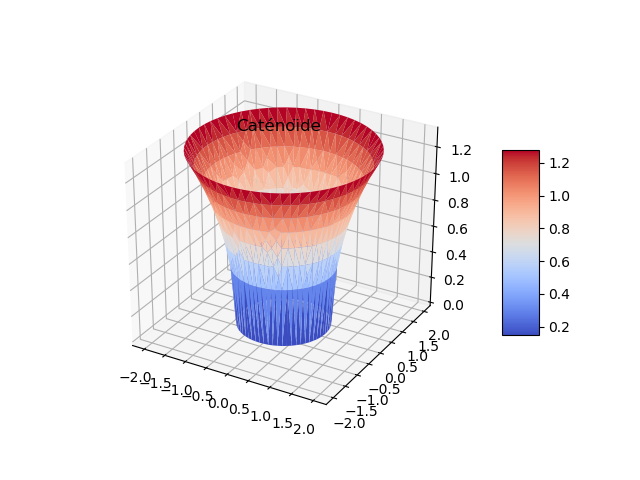
\includegraphics[width=\linewidth]{catenoide.png}
  %\caption{La cat\'eno\"ide.}
  %\label{fig:catenoide}

  \centering
  \subfloat[La cat\'eno\"ide.]{{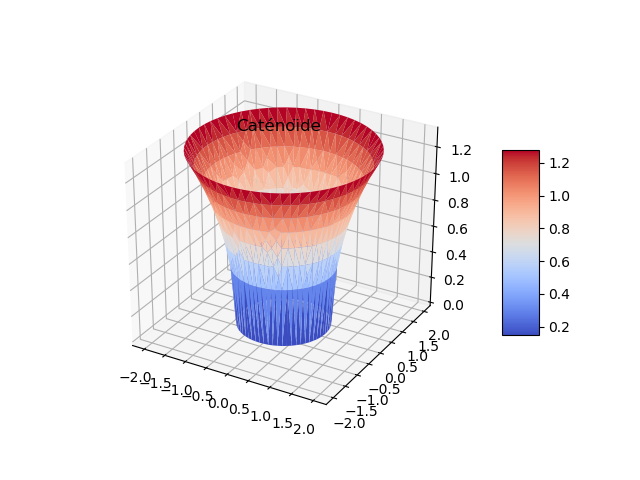
\includegraphics[width=\linewidth]{catenoide.png} }}%
  %\qquad
    \\
  \subfloat[$(x, y)\mapsto\cos(x)\cos(y)$]
    {{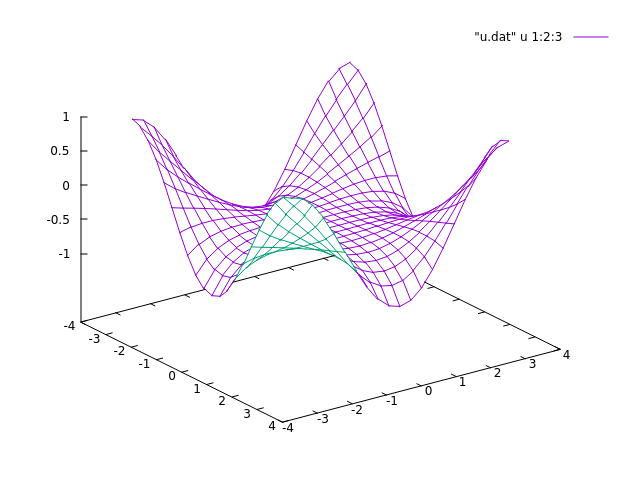
\includegraphics[width=\linewidth]{cos_cos.png} }}
  \caption{Les surfaces}
  \label{fig:example}
\end{figure}
\clearpage

\newpage

Q5) Voir code: test5.cpp . Voici les valeurs: \\
$$
\begin{array}{|c|c|c|}
\hline
\text{It\'eration} & \text{It\'eration du gradient} & \text{Erreur cons\'ecutive}
 \\
\hline
0 & 55 & 5.54098 \\
1 & 51 & 1.37066 \\
2 & 49 & 0.37741 \\
3 & 49 & 0.0963363 \\
4 & 48 & 0.0237973 \\
5 & 46 & 0.00588999 \\
6 & 44 & 0.00148339 \\
7 & 42 & 0.000383801 \\
8 & 40 & 0.000103052 \\
9 & 37 & 2.90305e^{-05} \\
10 & 35 & 8.64873e^{-06} \\
11 & 33 & 2.72588e^{-06} \\
12 & 31 & 9.01889e^{-07} \\
13 & 27 & 3.09612e^{-07} \\
14 & 22 & 1.09021e^{-07} \\
15 & 18 & 3.8991e^{-08} \\
16 & 8 & 1.39172e^{-08} \\
17 & 4 & 5.08228e^{-09} \\
18 & 3 & 1.90381e^{-09} \\
19 & 3 & 8.07361e^{-10} \\
20 & 1 & 2.32879e^{-10} \\
21 & 0 & 0 \\
\hline
\end{array}
$$

%\begin{figure}[h!]
%  \centering
%  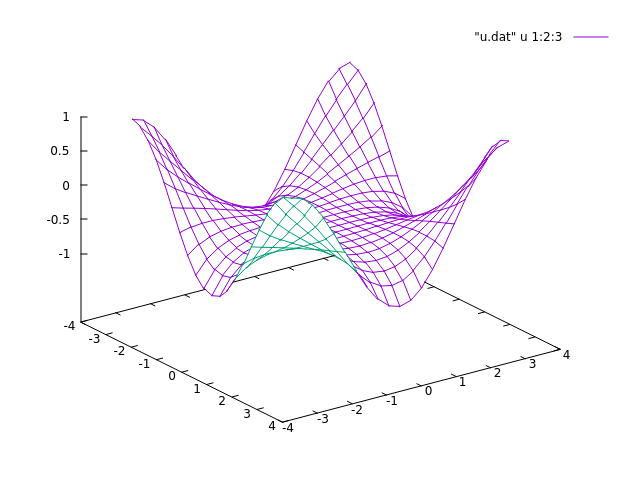
\includegraphics[width=\linewidth]{cos_cos.png}
%  \caption{$(x, y)\mapsto\cos(x)\cos(y)$.}
%  \label{fig:cos_cos}
%\end{figure}
%\clearpage

Q6) Quelques cas \\

\begin{figure}[h!]
  \centering
  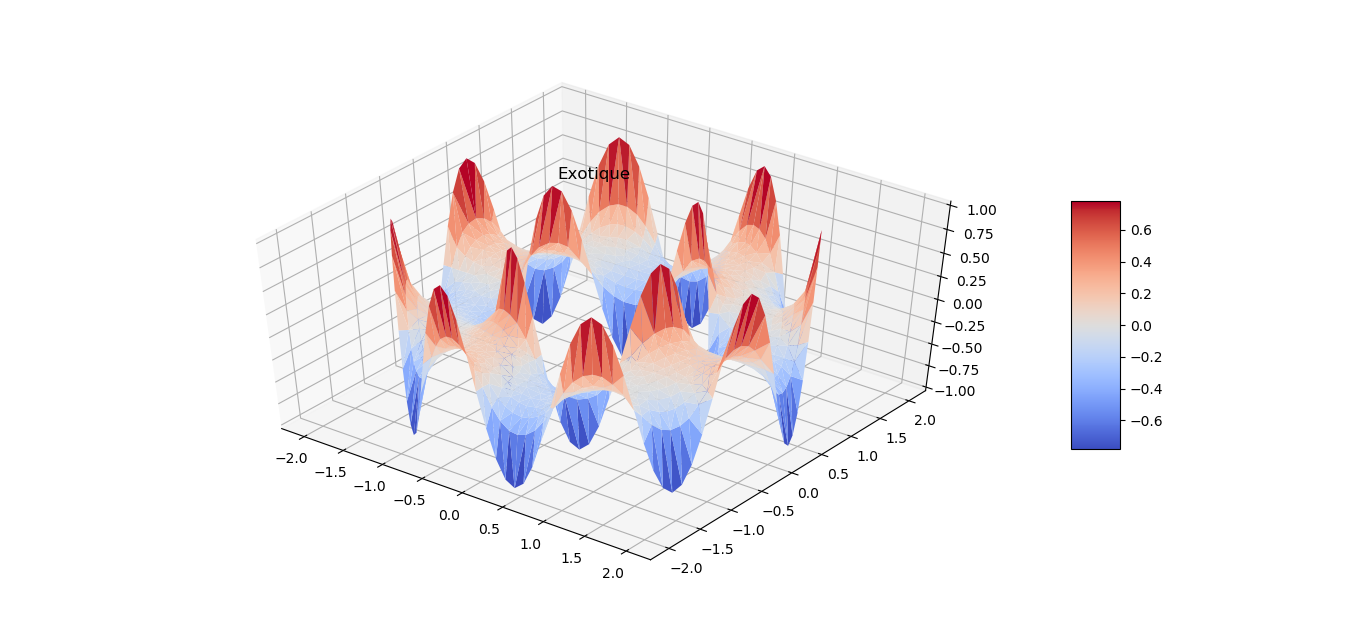
\includegraphics[width=\linewidth]{exotique.png}
  \caption{$(r, \theta)\mapsto\sin(4r\theta)$.}
  \label{fig:exotique}
\end{figure}
\clearpage

\newpage

\section{Conclusion}
Il y a plusieurs implementation possible pour r\'esoudre le probl\`eme de
 surface minimale en dimension finie.

Des id\'ees possibles pour am\'eliorer la performance seraient de conditionn\'ee
 la matrice $A$, faire de des calculs en parall\`ele en particulier pour la
 multiplication matrice-vecteur.

D'autres m\'ethodes pour la r\'esolution de syst\`emes num\'eriques peuvent
 \^etre utilis\'ees comme la factorisation LU, GMRes.

\newpage

\begin{thebibliography}{9}

%\bibitem{lamport94}
%  Leslie Lamport,
%  \textit{\LaTeX: a document preparation system},
%  Addison Wesley, Massachusetts,
%  2nd edition,
%  1994.

\bibitem{freefem++-doc}
  \url{https://github.com/FreeFem/FreeFem-doc-pdf/raw/master/freefem\%2B\%2Bdoc.pdf},

\bibitem{Eigen-doc}
  \url{http://eigen.tuxfamily.org/dox/}
\end{thebibliography}

\end{document}

